\documentclass{beamer}

\usepackage{amsmath}
\usepackage{amssymb}
\usepackage{booktabs}
\usepackage{epstopdf} %converting to PDF

\usetheme{AnnArbor}
\usecolortheme{beaver}

\mode<presentation>

\title{Overview of Results from Reggio}
%\author{P. Biroli et al.}
\date{\today}

\begin{document}

% Title Page
\begin{frame}
	\titlepage
\end{frame}

%\begin{frame}
%	\tableofcontents
%\end{frame}

\section{Data}
\subsection{Sample}

%%%%%%%%%%

\begin{frame}
	\frametitle{Cohort Structure}
	\begin{itemize}
	\item In each of the three cities (Reggio Emilia, Parma, and Padova), individuals in the following cohorts were interviewed.
	\end{itemize}
	\centering
	\vspace{1cm}
	\begin{tabular}{ccc}
	\toprule
	Cohort & Birth Year(s) & Age at Interview \\
	\midrule
	I & 1954-1959 & 54-60 years old  \\
	II & 1969-1971 & 43 years old \\
	III & 1981-1981 & 32 years old \\
	IV & 1994 & last year of compulsory schooling  \\
	V & 2006 & 1st year of elementary school  \\
	\bottomrule
	\end{tabular}
\end{frame}

%%%%%%%%%%

\begin{frame}
	\frametitle{Treatment and Control Structure}
Currently, this is the treatment and control structure. Note Cohort I was born before the implementation of the Reggio program.

	\vspace{0.2cm}
	\centering
	\footnotesize
	\begin{tabular}{ccccc}
	\toprule
	Cohort & \multicolumn{4}{c}{City} \\
	 & \multicolumn{2}{c}{Reggio} & Parma & Padova \\
	 & Municipal & Other & All & All \\
	\midrule
	I &  & C & C & C \\
	& & 200 & 103 & 146 \\
	II & T & C & C & C \\
	& 125 & 160 & 254 & 252 \\
	III & T & C & C & C \\
	& 143 & 137 & 251 & 251 \\
	IV & T & C & C & C \\
	& 156 & 144 & 254 & 282 \\
	V Ita. & T & C & C & C \\
	& 160 & 151 & 291 & 278 \\
	V Imm. & T & C & C & C \\
	&  70 &  40 &  58 & 113 \\
	\bottomrule
	\end{tabular}

{Response rate}:\ref{tab:RespRate}
\end{frame}

%%%%%%%%%%	

\begin{frame}
	\frametitle{Cohort Simplification}
	\begin{itemize}
		\item For this preliminary analysis, the cohorts will be simplified into:
		\begin{itemize}
			\item Child (Cohort V)
			\item Adolescent (Cohort IV)
			\item Adult (Cohorts I, II, III)
		\end{itemize}
	\end{itemize}
\end{frame}

%%%%%%%%%%	

\subsection{Variables for Analysis}

\begin{frame}
	\frametitle{Outcomes}
	To begin, we present results for the following outcomes:
	\begin{itemize}
		\item Strengths and Difficulties Questionnaire (SDQ) 
		\item Depression Scale
		\item In good health
		\item Bothered by migrants
	\end{itemize}
\end{frame}

%%%%%%%%%%

\begin{frame}
	\frametitle{Outcome Availability by Age Group}
	\centering
	\begin{tabular}{cccc}
	\toprule
	Outcome & \multicolumn{3}{c}{Age Group} \\ 
	\cmidrule{2-4}
	& Child & Adolescent & Adult \\
	\midrule
	Caregiver-reported SDQ & $\checkmark$ & $\checkmark$&  \\
	Individual-reported SDQ &  & $\checkmark$ &  \\
	\cmidrule{1-1}
	Caregiver-reported good health & $\checkmark$ & $\checkmark$ &  \\
	Individual-reported good health &  & $\checkmark$ & $\checkmark$ \\
	\cmidrule{1-1}
	Depression &  & $\checkmark$ & $\checkmark$ \\
	\cmidrule{1-1}
	Bothered by migrants & & $\checkmark$& $\checkmark$ \\
	\bottomrule
	\end{tabular}
\end{frame}

%%%%%%%%%%

\section{Analysis}

\subsection{Raw Data}
\begin{frame}
The following plots show the raw-average for the variable of interest, split by City and Preschool type.
\end{frame}

\begin{frame}
\center
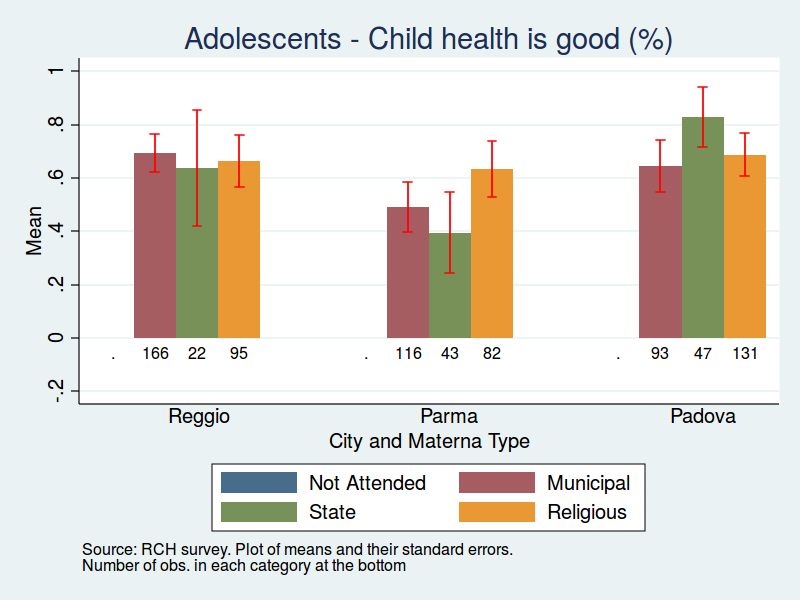
\includegraphics[scale=0.40]{../pietro/Tables/childHealthPerc_Ado.png}
\end{frame}

\subsection{Controls Considered}

%%%%%%%%%%

\begin{frame}
	\frametitle{Controls Considered}
	\begin{itemize}
		\item Gender, age at interview, age$^2$
	\end{itemize}
Dummies for: 
	\begin{itemize}
		\item Parental education
		\item Parents born in the region (province)
		\item Caregiver attended preschool
		\item Family owns home, family income brackets
		\item Low birthweight, born premature	
		\item Interviewer f.e., interview mode (computer or paper)
	\end{itemize}
\end{frame}

%%%%%%%%%%

\subsection{Tables of Results}

%%%%%%%%%%

\subsubsection{Strengths \& Difficulties}
\begin{frame}
\center
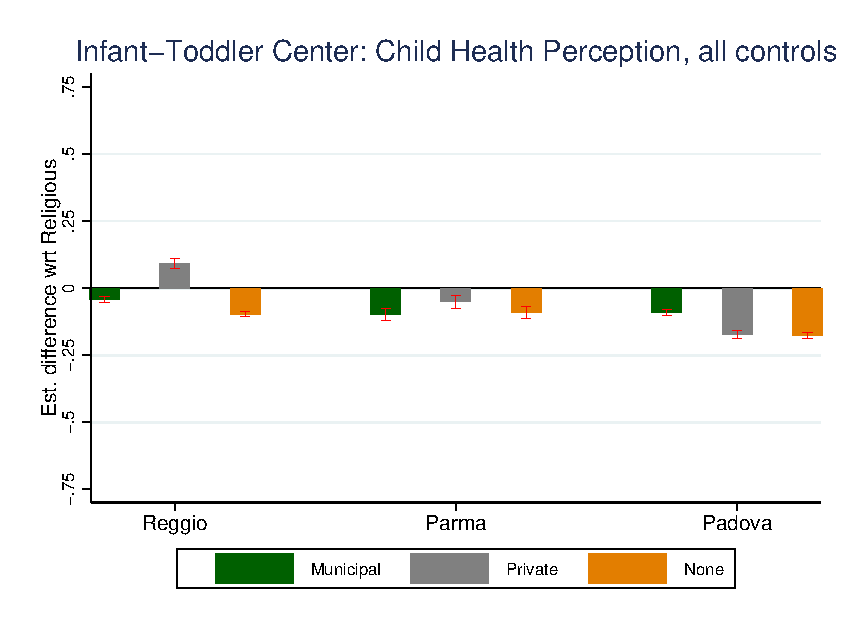
\includegraphics[scale=0.7]{../Output/graphs/CH_Asilo_Child_all.eps}
\end{frame}

%%%%%%%%%%

\appendix

\begin{frame}
\center
\huge
Additional Tables
\end{frame}

\begin{frame}
\begin{tiny}
%\begin{table}[ht!]
\caption{\textbf{Completed Interviews and Response Rates}}
%\footnotesize
\label{tab:RespRate}
\begin{center}
\begin{tabular}{ l | c | c | c | c | c }
\hline\hline
\textbf{Cohort} & \multicolumn{2}{c}{\textbf{Reggio}} & \textbf{Parma} & \textbf{Padova} & \textbf{Total}\\
\hline
Children (yob 2006)       & Mun. & Rel.+St.+NoP. & Mun.+Rel.+St.+NoP. & Mun.+Rel.+St.+NoP.&\\[0.2em]
Italian (Cohort V)          & 160  & 151            & 291                & 278               & 880\\[0.2em]
\hline
\textit{Nov.2012-Aug.2013} & \multicolumn{2}{c|}{\textit{RR: 50.1\%}} & \textit{RR: 62.7\%} & \textit{RR: 50.1\%} & \textit{RR: 53.6\%}\\[0.2em]
\hline
Children (yob 2006)       & Mun. & Rel.+St.+NoP. & Mun.+Rel.+St.+NoP. & Mun.+Rel.+St.+NoP.&\\[0.2em]
Immigrant (Cohort V)        & 70   & 40             & 58                 & 113               & 281\\[0.2em]
\hline
\textit{Nov.2012-Aug.2013} & \multicolumn{2}{c|}{\textit{RR: 53.1\%}} & \textit{RR: 49.2\%} & \textit{RR: 63.1\%} & \textit{RR: 55.8\%}\\[0.2em]
\hline
Adolescents (yob 1994)    & Mun. & Rel.+St.+NoP. & Mun.+Rel.+St.+NoP. & Mun.+Rel.+St.+NoP.&\\[0.2em]
(Cohort IV)                 & 156  & 144            & 254                & 282               & 836\\[0.2em]
\hline
\textit{Nov.2012-Jul.2013} & \multicolumn{2}{c|}{\textit{RR: 57.1\%}} & \textit{RR: 58.5\%} & \textit{RR: 55.5\%} & \textit{RR: 57.0\%}\\[0.2em]
\hline
Adults (yob 1980-81)       & Mun. & Rel.+St.+NoP. & Mun.+Rel.+St.+NoP. & Mun.+Rel.+St.+NoP.&\\[0.2em]
(Cohort III)                 & 143  & 137            & 251                & 251               & 782\\[0.2em]
\hline
\textit{May 2013-Nov.2013} & \multicolumn{2}{c|}{\textit{RR: 58.3\%}} & \textit{RR: 58.2\%} & \textit{RR: 57.4\%} & \textit{RR: 58.0\%}\\[0.2em]
\hline
Adults (yob 1969-70)        & Mun. & Rel.+St.+NoP. & Mun.+Rel.+St.+NoP. & Mun.+Rel.+St.+NoP.&\\[0.2em]
(Cohort II)                   & 125  & 160            & 254                & 252               & 791\\[0.2em]
\hline
\textit{May 2013-Nov.2013} & \multicolumn{2}{c|}{\textit{RR: 59.3\%}} & \textit{RR: 56.3\%} & \textit{RR: 57.5\%} & \textit{RR: 57.7\%}\\[0.2em]
\hline
Adults (yob 1954-59)     & \multicolumn{2}{c|}{Mun.+Rel.+St.+NoP.} & Mun.+Rel.+St.+NoP. & Mun.+Rel.+St.+NoP.&\\[0.2em]
(Cohort I)                 & \multicolumn{2}{c|}{200} & 103 & 146 & 449\\[0.2em]
\hline
\textit{May 2013-Oct.2013} & \multicolumn{2}{c|}{\textit{RR: 52.2\%}} & \textit{RR: 63.6\%} & \textit{RR: 62.7\%} & \textit{RR: 57.7\%}\\[0.2em]
\hline 
\textbf{Total Interviews} & \multicolumn{2}{c|}{\textbf{1,486}} & \textbf{1,211} & \textbf{1,322} & \textbf{4,019} \\[0.2em]
\textit{Total Response Rates}       & \multicolumn{2}{c|}{\textit{55.1\%}} & \textit{58.8\%} & \textit{56.2\%} & \textit{56.5\%} \\
\hline
\end{tabular}
\end{center}
%\footnotesize
\tiny{{\bfseries Notes:} Mun.=Municipal Preschool; Rel.=Religious Preschool; St.=State Preschool; NoP.=No Preschool attended. yob=year of birth. For each cohort, the third line in the first column reports the interview periods. RR=response rate. The response rates are calculated as the ratio of interviews to total valid contacts. Valid contacts are the sum of: completed interviews, sharp refusal, no person present, talked with a relative, left paper questionnaire but never returned, interview began but not completed.}
\end{table} 
\begin{table}[ht!]
\caption{\textbf{Completed Interviews and Response Rates}}
%\footnotesize
\label{tab:RespRate}
\begin{center}
\begin{tabular}{ l | c | c | c | c | c }
\hline\hline
\textbf{Cohort} & \multicolumn{2}{c}{\textbf{Reggio}} & \textbf{Parma} & \textbf{Padova} & \textbf{Total}\\
\hline
Children (yob 2006)       & Mun. & Rel.+St.+NoP. & Mun.+Rel.+St.+NoP. & Mun.+Rel.+St.+NoP.&\\[0.2em]
Italian (Cohort V)          & 160  & 151            & 291                & 278               & 880\\[0.2em]
\hline
\textit{Nov.2012-Aug.2013} & \multicolumn{2}{c|}{\textit{RR: 50.1\%}} & \textit{RR: 62.7\%} & \textit{RR: 50.1\%} & \textit{RR: 53.6\%}\\[0.2em]
\hline
Children (yob 2006)       & Mun. & Rel.+St.+NoP. & Mun.+Rel.+St.+NoP. & Mun.+Rel.+St.+NoP.&\\[0.2em]
Immigrant (Cohort V)        & 70   & 40             & 58                 & 113               & 281\\[0.2em]
\hline
\textit{Nov.2012-Aug.2013} & \multicolumn{2}{c|}{\textit{RR: 53.1\%}} & \textit{RR: 49.2\%} & \textit{RR: 63.1\%} & \textit{RR: 55.8\%}\\[0.2em]
\hline
Adolescents (yob 1994)    & Mun. & Rel.+St.+NoP. & Mun.+Rel.+St.+NoP. & Mun.+Rel.+St.+NoP.&\\[0.2em]
(Cohort IV)                 & 156  & 144            & 254                & 282               & 836\\[0.2em]
\hline
\textit{Nov.2012-Jul.2013} & \multicolumn{2}{c|}{\textit{RR: 57.1\%}} & \textit{RR: 58.5\%} & \textit{RR: 55.5\%} & \textit{RR: 57.0\%}\\[0.2em]
\hline
Adults (yob 1980-81)       & Mun. & Rel.+St.+NoP. & Mun.+Rel.+St.+NoP. & Mun.+Rel.+St.+NoP.&\\[0.2em]
(Cohort III)                 & 143  & 137            & 251                & 251               & 782\\[0.2em]
\hline
\textit{May 2013-Nov.2013} & \multicolumn{2}{c|}{\textit{RR: 58.3\%}} & \textit{RR: 58.2\%} & \textit{RR: 57.4\%} & \textit{RR: 58.0\%}\\[0.2em]
\hline
Adults (yob 1969-70)        & Mun. & Rel.+St.+NoP. & Mun.+Rel.+St.+NoP. & Mun.+Rel.+St.+NoP.&\\[0.2em]
(Cohort II)                   & 125  & 160            & 254                & 252               & 791\\[0.2em]
\hline
\textit{May 2013-Nov.2013} & \multicolumn{2}{c|}{\textit{RR: 59.3\%}} & \textit{RR: 56.3\%} & \textit{RR: 57.5\%} & \textit{RR: 57.7\%}\\[0.2em]
\hline
Adults (yob 1954-59)     & \multicolumn{2}{c|}{Mun.+Rel.+St.+NoP.} & Mun.+Rel.+St.+NoP. & Mun.+Rel.+St.+NoP.&\\[0.2em]
(Cohort I)                 & \multicolumn{2}{c|}{200} & 103 & 146 & 449\\[0.2em]
\hline
\textit{May 2013-Oct.2013} & \multicolumn{2}{c|}{\textit{RR: 52.2\%}} & \textit{RR: 63.6\%} & \textit{RR: 62.7\%} & \textit{RR: 57.7\%}\\[0.2em]
\hline 
\textbf{Total Interviews} & \multicolumn{2}{c|}{\textbf{1,486}} & \textbf{1,211} & \textbf{1,322} & \textbf{4,019} \\[0.2em]
\textit{Total Response Rates}       & \multicolumn{2}{c|}{\textit{55.1\%}} & \textit{58.8\%} & \textit{56.2\%} & \textit{56.5\%} \\
\hline
\end{tabular}
\end{center}
%\footnotesize
\tiny{{\bfseries Notes:} Mun.=Municipal Preschool; Rel.=Religious Preschool; St.=State Preschool; NoP.=No Preschool attended. yob=year of birth. For each cohort, the third line in the first column reports the interview periods. RR=response rate. The response rates are calculated as the ratio of interviews to total valid contacts. Valid contacts are the sum of: completed interviews, sharp refusal, no person present, talked with a relative, left paper questionnaire but never returned, interview began but not completed.}
\end{table} 
\end{tiny}
\end{frame}

\end{document}